\documentclass[10pt,a4paper,twoside]{article}

% Page layout
\usepackage[a4paper,margin=2.3cm]{geometry}
\usepackage{setspace}
\usepackage{parskip}

% Mathematics and tables
\usepackage{amsmath}
\usepackage{amssymb}
\usepackage{booktabs}
\usepackage{array}

% Figures and captions
\usepackage{graphicx}
\usepackage[font=small,labelfont=bf]{caption}
\usepackage{subcaption}
\usepackage{placeins}
\graphicspath{{Figures/}}


% Code listings
\usepackage{xcolor}
\usepackage{listings}

% References and links
\usepackage[numbers]{natbib}
\usepackage[hidelinks]{hyperref}
\usepackage[nameinlink,noabbrev]{cleveref}

\definecolor{codebackground}{RGB}{247,249,252}
\definecolor{codecomment}{RGB}{80,120,80}
\definecolor{codekeyword}{RGB}{25,73,145}
\definecolor{codestring}{RGB}{145,65,25}

\lstdefinestyle{reportcode}{
    basicstyle=\ttfamily\footnotesize,
    keywordstyle=\color{codekeyword},
    commentstyle=\color{codecomment},
    stringstyle=\color{codestring},
    backgroundcolor=\color{codebackground},
    frame=single,
    rulecolor=\color{black!20},
    breaklines=true,
    columns=fullflexible,
    keepspaces=true,
    showstringspaces=false,
    tabsize=4
}
\lstset{style=reportcode}

\title{\textbf{Image Segmentation Using Contextual Features}\\
\large }


\author{
    \begin{tabular}{c c}
        Lars Heijnen & Amir Rezaei \\
        Student ID: 2233878 & Student ID: 2294753 \\
        [2em] % Adds vertical space between rows
        Emery de Korte & Lynk Koh \\
        Student ID: 1872729 & Student ID: 2413078 \\
    \end{tabular}
}
\date{\today}

\begin{document}

\maketitle


\tableofcontents
\newpage
\section{Introduction}

Brain tissue segmentation converts MR images into anatomical tissue regions that can be measured and compared between subjects. In this project, the aim was to segment each pixel into one of four classes: background/other, white matter, gray matter, or cerebrospinal fluid (CSF).

This is difficult to do from raw intensity alone. T1 and T2 images contain useful tissue information, but the tissue classes partly overlap in intensity space. A single pixel intensity also does not describe local image context, such as whether the pixel lies in a homogeneous tissue region, near a boundary, or closer to the image center. For this reason, the course material motivates segmentation in feature space, where each pixel is represented by multiple intensity, texture, edge, and spatial features before classification~\cite{su2026featurespace}.

The main research question was: \textit{Does progressively adding contextual features improve multi-class brain tissue segmentation compared with using only raw T1/T2 intensity?}

The hypothesis was that contextual features would improve segmentation performance. Gaussian-smoothed intensities were expected to add neighborhood information, gradient features to add boundary information, the distance-to-center feature to add spatial information, and local standard deviation to add texture information. We therefore expected multi-class Dice to increase and classification error to decrease as these feature groups were added.

\section{Study Design}

The experiment used the provided MRBrainS image data. For each subject and slice, a T1 image, a T2 image, and a ground-truth label image were available. The original labels were converted into four tissue classes: background/other, white matter, gray matter, and cerebrospinal fluid (CSF). The exact mapping is shown in Appendix~\ref{app:label-mapping}. This made the task a multi-class tissue segmentation problem.

The main research question was tested with a feature ablation study. The classifier was kept fixed as k-nearest neighbors (kNN) with $k=3$, while the amount of contextual image information was progressively increased. This design makes the comparison easier to interpret, because changes in performance can mainly be attributed to the added feature groups rather than to changes in classifier type or model complexity.

Subjects 1, 2, and 3 were used for training, while subjects 4 and 5 were used for testing. All three available slices were included for each subject, giving nine training subject-slice pairs and six test subject-slice pairs. A subject-level split was used instead of splitting pixels randomly across the full dataset, because this better tests whether the method generalizes to unseen subjects.

For each subject and slice, 11 features were extracted per pixel. Pixels were sampled in a class-balanced way, with at most 600 pixels per class per image, to reduce computation time and limit dominance of the background class.

For every feature set, the test features were normalized using the training-set mean and standard deviation. Performance was evaluated with multi-class Dice as the main overlap metric and classification error as a complementary pixel-wise measure.

In addition to the open-ended feature ablation experiment, the closed-ended notebook work compared single kNN, combined kNN, and our custom combined method on slice 1 using a leave-one-subject-out setup over the five subjects. This comparison was used to evaluate whether combining several kNN-based predictions improved segmentation performance compared with a single kNN classifier.
\section{Methods}

\subsection{Feature extraction}

For each subject and slice, the T1 image, T2 image, and ground-truth image were loaded from the provided MRBrainS data. The feature extraction was implemented in \texttt{segmentation\_util.py}. Each image was converted to floating point values before the derived image features were computed.

The first two features were the raw T1 and T2 pixel intensities. Gaussian-smoothed intensity features were then computed for both modalities using Gaussian filters with $\sigma = 1$ and $\sigma = 3$. This resulted in four smoothed intensity features: T1 at $\sigma = 1$, T1 at $\sigma = 3$, T2 at $\sigma = 1$, and T2 at $\sigma = 3$.

Gradient magnitude features were computed for both T1 and T2 using a Gaussian gradient magnitude filter with $\sigma = 1$. These features were included to represent local edge strength, which is relevant near tissue boundaries.

A spatial feature was added by computing the Euclidean distance from each pixel to the image center. For a pixel at row $r$ and column $c$, this feature was computed as

\[
d(r,c) = \sqrt{(r-r_c)^2 + (c-c_c)^2},
\]

where $r_c$ and $c_c$ are the row and column coordinates of the image center. This gives the classifier simple spatial information without using the ground-truth labels.

The custom texture feature was local standard deviation. In the implementation, this was computed by first applying a Gaussian filter with $\sigma = 2$ to the image and to the squared image. The local variance was then calculated as

\[
\sigma_{\mathrm{local}}^2 = G_{\sigma=2}(I^2) - G_{\sigma=2}(I)^2,
\]

where $G_{\sigma=2}$ denotes Gaussian smoothing with $\sigma = 2$. Negative numerical values were clipped to zero, and the square root was taken to obtain the local standard deviation. This feature was computed for both T1 and T2. It measures local intensity variation and was used as a simple texture descriptor.

In total, the implementation produced 11 features per pixel: T1 intensity, T2 intensity, four Gaussian-smoothed intensity features, two gradient magnitude features, distance to the image center, and two local standard deviation features.

\subsection{Open-ended feature ablation experiment}

The open-ended experiment tested whether contextual features improve tissue segmentation compared with raw intensity features alone. The experiment was implemented in the segmentation project notebook. The classifier was kept fixed as k-nearest neighbors (kNN) with $k=3$ for all feature sets.

The subject-level split described in the study design was used: subjects 1--3 for training and subjects 4--5 for testing, using all three slices per subject. From each subject-slice pair, at most 600 pixels per class were sampled for both training and testing.

The feature sets were cumulative: raw T1/T2 intensity was used as the baseline, followed by Gaussian-smoothed intensities, T1 local standard deviation, gradient magnitudes, distance-to-center, and T2 local standard deviation.

For every feature set, the training data were normalized by subtracting the training mean and dividing by the training standard deviation. The same training mean and standard deviation were then used to normalize the test data. This was done because kNN uses Euclidean distances, and features with larger numerical scales would otherwise have more influence on the nearest-neighbor calculation.

After normalization, a \texttt{KNeighborsClassifier} with $k=3$ was fitted on the sampled training pixels and applied to the sampled test pixels. The predicted labels were compared with the ground-truth tissue labels using classification error and multi-class Dice.

\subsection{Closed-ended method comparison}

In addition to the open-ended feature ablation experiment, the notebook also compared three segmentation approaches on slice 1 using all five subjects. In this experiment, each subject was used once as the test subject, while the other four subjects were used for training. This created a leave-one-subject-out comparison over the five subjects.

The first method was a single kNN classifier. In the implementation, this method used one training subject and applied \texttt{segmentation\_knn} with $k=3$. The \texttt{segmentation\_knn} function randomly sampled 3000 training pixels, normalized the sampled training data and test data using the sampled training statistics, and then fitted a kNN classifier.

The second method was combined kNN. This method trained one kNN classifier for each training subject and combined the predicted labels by majority voting. The implementation preserves the multi-class tissue labels, so the predictions remain labels 0, 1, 2, and 3 instead of being converted to binary labels.

The third method was the custom method, implemented as \texttt{segmentation\_mymethod}. This method combined several predictions by majority voting. The predictions included combined kNN, pooled kNN using all features with $k=3$, pooled kNN using all features with $k=7$, and additional pooled kNN predictions using selected contextual feature views. The pooled kNN predictions used balanced class sampling with up to 500 pixels per class. After majority voting, a $3 \times 3$ local majority filter was applied to the predicted label image as a simple spatial smoothing step.

\subsection{Evaluation metrics}

Segmentation performance was evaluated using classification error and multi-class Dice. Classification error was computed as the mean fraction of pixels for which the predicted label differed from the ground-truth label.

Multi-class Dice was computed by treating each class as foreground once and all other classes as background. The binary Dice scores for the individual classes were then averaged. This gives one overlap score for the full multi-class tissue segmentation.


\section{Results}

\subsection{Contextual Feature Ablation}

The open-ended feature ablation experiment showed a consistent improvement when contextual features were added to the raw T1/T2 intensity features. Multi-class Dice increased from 0.7260 for the baseline intensity-only feature set to 0.8245 when all available contextual features were used, while classification error decreased from 0.2691 to 0.1749. The numerical results are shown in Table~\ref{tab:feature-ablation-results}, and the same trend is visualized in Figure~\ref{fig:feature-ablation-results}.

\begin{table}[t]
\centering
\caption{Performance of the cumulative feature sets in the open-ended kNN experiment. All models used kNN with $k=3$.}
\label{tab:feature-ablation-results}
\begin{tabular}{lrrrr}
\toprule
Feature set & Features & Dice & Dice gain & Error \\
\midrule
T1/T2 intensity & 2 & 0.7260 & 0.0000 & 0.2691 \\
+ Gaussian smoothing & 6 & 0.7542 & 0.0282 & 0.2421 \\
+ T1 local texture & 7 & 0.7653 & 0.0393 & 0.2291 \\
+ gradients & 9 & 0.7920 & 0.0660 & 0.2066 \\
+ distance to center & 10 & 0.8188 & 0.0929 & 0.1804 \\
+ T2 local texture & 11 & 0.8245 & 0.0985 & 0.1749 \\
\bottomrule
\end{tabular}
\end{table}

\begin{figure}[t]
\centering
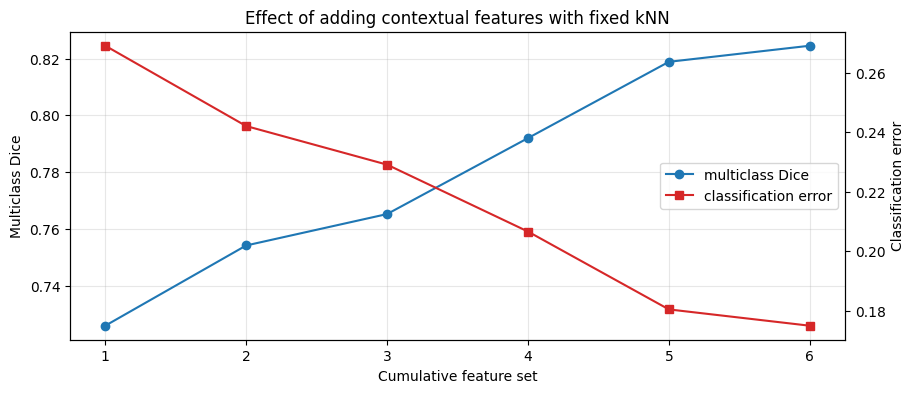
\includegraphics[width=0.82\linewidth]{figures/context_feature_ablation.png}
\caption{Feature ablation results for the open-ended research question.}
\label{fig:feature-ablation-results}
\end{figure}


The largest gains were observed after adding Gaussian-smoothed intensity features, gradient features, and the distance-to-center feature. The final T2 local texture feature also improved the result, but the additional gain was smaller than for the earlier contextual feature groups.

\subsection{Combined kNN and Custom Method}

The closed-ended method comparison was evaluated on slice 1 in a leave-one-subject-out setup over the five subjects. The mean scores are shown in Table~\ref{tab:method-comparison-results}. The combined kNN method gave the lowest mean classification error, while our custom method gave the highest mean multi-class Dice.

\begin{table}[t]
\centering
\caption{Mean tissue segmentation performance over the five leave-one-subject-out experiments on slice 1.}
\label{tab:method-comparison-results}
\begin{tabular}{lrr}
\toprule
Method & Classification error & Multi-class Dice \\
\midrule
Single kNN & 0.1240 & 0.7458 \\
Combined kNN & 0.1193 & 0.7580 \\
Our method & 0.1254 & 0.7657 \\
\bottomrule
\end{tabular}
\end{table}

Compared with the single kNN classifier, combined kNN improved both mean classification error and Dice. Our method further improved Dice from 0.7580 to 0.7657 compared with combined kNN, but its classification error was slightly higher at 0.1254. This means that the custom method improved average region overlap, while not being the best method according to pixel-wise error.

Subject 1 was the clearest positive example for our method. It reached Dice 0.8173, compared with 0.7951 for combined kNN and 0.7679 for single kNN. Subject 2 was a weaker case: our method reached Dice 0.7681, below combined kNN at 0.7962. These two examples are shown in Figure~\ref{fig:method-comparison-examples}.

\begin{figure}[t]
\centering
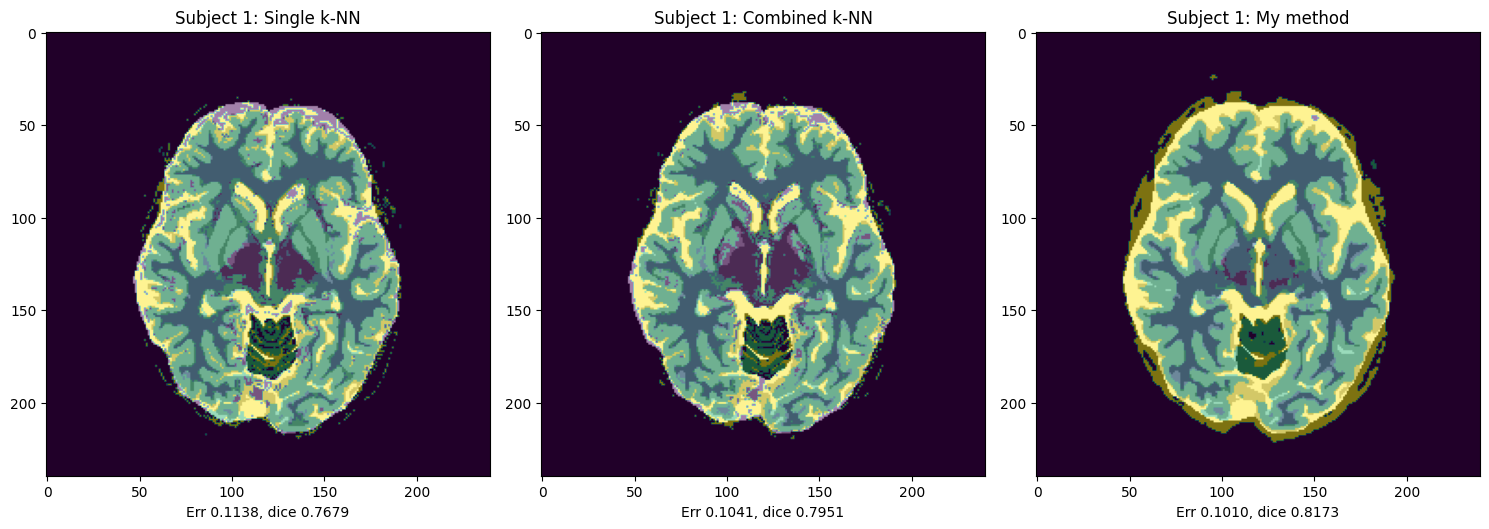
\includegraphics[width=0.82\linewidth]{figures/section3_subject_1.png}

\vspace{0.4em}

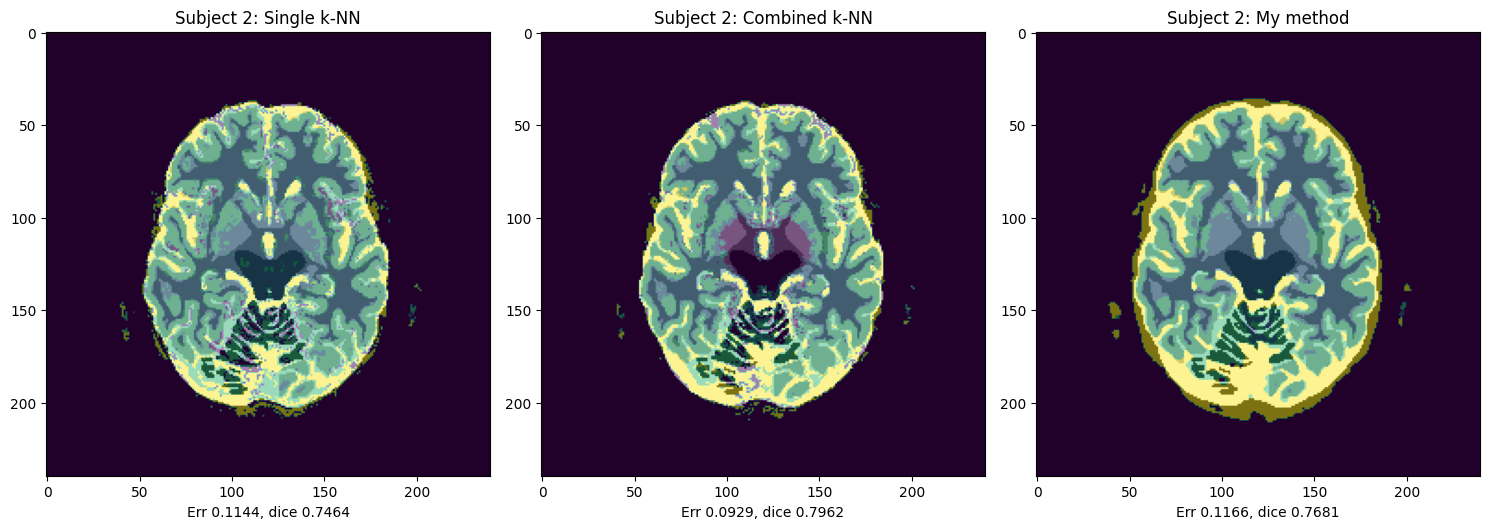
\includegraphics[width=0.82\linewidth]{figures/section3_subject_2.png}
\caption{Example segmentations for subject 1 and subject 2 in the method comparison.}
\label{fig:method-comparison-examples}
\end{figure}

\section{Discussion}

The results support the hypothesis that contextual features improve kNN-based tissue segmentation compared with raw T1/T2 intensity alone. In the feature ablation experiment, every added feature group increased the multi-class Dice score and reduced the classification error. The best feature set used all available contextual features, increasing Dice from 0.7260 to 0.8245. This suggests that the additional features did not only add redundant dimensions, but provided useful information about local image context and spatial structure.

The improvement from Gaussian smoothing is expected, because tissue regions are spatially coherent and a smoothed intensity value contains neighborhood information that a single raw pixel does not. The improvement after adding gradient features suggests that boundary information is useful for separating tissue classes. The distance-to-center feature also improved performance, probably because the images are similarly positioned and the main tissue classes have a broad spatial organization in these slices. However, this feature is also one of the less general features. If the images were less well aligned, or if slices came from different anatomical levels, the same distance feature could become less reliable.

The local standard deviation features gave a smaller improvement than smoothing, gradients, and location. This is still a useful result. Local standard deviation measures local intensity variation, so part of its information overlaps with gradients and smoothed intensities. The fact that it still improved the final result shows that it added some complementary texture information, but it was not the main driver of the performance gain.

The method-comparison experiment gives a second insight. Combined kNN improved over single kNN, which suggests that majority voting across subject-specific classifiers can reduce dependence on one training subject. Our custom method achieved the highest mean Dice score, but it did not achieve the lowest classification error. This means it should not be described as clearly better on all metrics. It improved average region overlap, which is important for segmentation, but the slightly worse classification error shows that the local voting and smoothing steps can also introduce wrong pixel labels. The subject 2 result supports this limitation, since the custom method performed worse than combined kNN for that case.

A strength of the study is that the main experiment used a subject-level train-test split. This is more meaningful than testing on pixels from the same subject, because it evaluates whether the method generalizes to unseen subjects. Another strength is that the feature ablation was systematic: the classifier, value of $k$, normalization procedure, and train-test split were kept fixed, while only the feature set was changed. This makes the effect of adding contextual features easier to interpret.

There are also important limitations. The dataset is small, with five subjects and three slices per subject. The open-ended experiment used one fixed split, with subjects 1--3 for training and subjects 4--5 for testing. The results therefore show a clear trend for this split, but they do not prove that the exact same ordering would hold for every possible subject split. The balanced pixel sampling strategy was useful for computation time and class balance, but it means that not every available pixel was used for training or evaluation. The results can therefore still depend on the sampled pixels and should ideally be repeated with multiple random seeds.

Further analysis could include leave-one-subject-out evaluation for the feature ablation experiment, repeated balanced samples, and per-class Dice scores. Per-class Dice would be especially useful because the current mean Dice summarizes all tissue classes, while some tissues may benefit more from contextual features than others. A more advanced spatial method could also be tested, for example a graph-cut or CRF-style method~\cite{scannell2026graphcuts} using classifier probabilities as the data term and image gradients as the smoothness term. This would connect more directly to the spatial segmentation methods from the course than the simple local majority filter used here.

Overall, the project shows that contextual features improve multi-class brain tissue segmentation in this dataset. The clearest methodological insight is that raw intensity features are useful but incomplete: smoothing, boundary information, spatial position, and local texture each add information that helps kNN classify tissue pixels. At the same time, the results should be interpreted with care because the dataset is small and the best-performing custom method was not best on every metric.

\section{Contributions}

\begin{itemize}
    \item \textbf{Lars Heijnen:} Completed Section 1 and the related dependencies for Section 1. Collaborated on the research question. Completed Section 3 and helped with the open-ended project work, especially the representation of the data. Wrote the main body of the report and revised both the code and the report.

    \item \textbf{Amir Rezaei:} Completed Section 2 and wrote the Python implementation for the open-ended project work. Provided minor support for Section 3. Collaborated on the research question, helped complete the report, and revised both the code and the report.

    \item \textbf{Emery de Korte:} Wrote an initial version of the introduction, methods, and study design sections of the report, which were not complete and not used in the current report. Collaborated on the research question.

    \item \textbf{Lynk Koh:} Collaborated on the research question.
\end{itemize}

\section{LLM Usage Declaration}

Large language models were used during the project to support plotting of the results, optimization and cleaning of the code structure, and checking the grammar and structure of comments.

\appendix

\section{Label Mapping}
\label{app:label-mapping}

\begin{table}[h]
\centering
\caption{Mapping from the original MRBrainS ground-truth labels to the four tissue classes used in this project.}
\label{tab:label-mapping}
\begin{tabular}{lll}
\toprule
New label & Tissue class & Original labels \\
\midrule
0 & Background/other & 0, 1, 6 \\
1 & White matter & 2, 5 \\
2 & Gray matter & 3, 7 \\
3 & CSF & 4, 8 \\
\bottomrule
\end{tabular}
\end{table}


\bibliographystyle{IEEEtranN}
\bibliography{References}

\end{document}